\normaltrue
\correctiontrue

%\UPSTIidClasse{11} % 11 sup, 12 spé
%\newcommand{\UPSTIidClasse}{12}


\exer{Mouvement TT -- $\star$ \label{B2:13:03:02}}
\setcounter{question}{0}\marginnote{\UPSTIcompetence{B2-13}}
\index{Compétence B2-13}
\index{Mécanisme à 2 translations}
\ifcorrection
\else
\marginnote{\textbf{Pas de corrigé pour cet exercice.}}
\fi

\ifprof
\else
Soit le mécanisme suivant. On note $\vect{AB}=\lambda(t)\vect{i_0}$ et $\vect{BC}=\mu(t)\vect{j_0}$.
\begin{center}
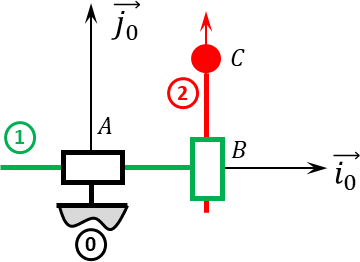
\includegraphics[width=.5\linewidth]{03_TT_01}
\end{center}
\fi

% ===============
\ifprof
\else
\marginnote{
\begin{solution}
\begin{enumerate}
\item $\vectv{C}{2}{0} =  \dot{\lambda}(t)\vect{i_0}+\dot{\mu}(t)\vect{j_0}$.
\item $\torseurcin{V}{2}{0}= \torseurl{\vect{0}}{\dot{\lambda}(t)\vect{i_0}+\dot{\mu}(t)\vect{j_0}}{\forall P}$.
\item $\vectg{C}{2}{0} = \ddot{\lambda}(t)\vect{i_0}+\ddot{\mu}(t)\vect{j_0}$.
\end{enumerate} 
\end{solution}
Corrigé  voir \ref{B2:13:03:02}.}
\fi
% ===============

\question{Déterminer $\vectv{C}{2}{0}$ par dérivation vectorielle ou par composition.}
\ifprof~\\ 

Par dérivation vectorielle, on a : $\vectv{C}{2}{0} $
$ = \deriv{\vect{AC}}{\rep{0}}$
$ = \dot{\lambda}(t)\vect{i_0}+\dot{\mu}(t)\vect{j_0}$.

Par composition du torseur cinématique, on a : 
$\vectv{C}{2}{0} = \vectv{C}{2}{1} +\vectv{C}{1}{0}$
$ = \deriv{\vect{BC}}{\rep{1}}+\deriv{\vect{AC}}{\rep{0}}$
$ = \dot{\lambda}(t)\vect{i_0}+\dot{\mu}(t)\vect{j_0}$.
\else
\fi

\question{Donner le torseur cinématique $\torseurcin{V}{2}{0}$ au point $C$.}
\ifprof ~\\
$\torseurcin{V}{2}{0}= \torseurl{\vect{0}}{\dot{\lambda}(t)\vect{i_0}+\dot{\mu}(t)\vect{j_0}}{\forall P}$.
\else
\fi

\question{Déterminer $\vectg{C}{2}{0}$.}
\ifprof ~\\
 $\vectg{C}{2}{0} = \deriv{\vectv{C}{2}{0}}{\rep{0}}=\ddot{\lambda}(t)\vect{i_0}+\ddot{\mu}(t)\vect{j_0}$.
\else
\fi




